\documentclass[a4paper,12pt]{article}
%\usepackage[latin1]{inputenc}
\usepackage[spanish]{babel}
\usepackage{graphicx}
\usepackage{amsmath}
\spanishdecimal{.}
\usepackage{wrapfig}
\setlength{\textheight}{250mm}
\setlength{\textwidth}{165mm}
\setlength{\topmargin}{-15mm}
\setlength{\oddsidemargin}{0pt}
\pagestyle{empty}

\begin{document}

\def\bm#1{{\mbox{\boldmath $#1$}}}
\def\eqdef{\buildrel \rm def \over =}
\def\signo{\mathop{\rm signo}\nolimits}

\mbox{}\vspace*{-20mm}

{\centering
{\small\sc Escuela Técnica Superior de Ingenieros de Caminos, Canales y Puertos (Madrid)}\\*[4mm]
{\Large\bf Método de los Elementos Finitos 23-24}\\*[4mm]
PRÁCTICA 5. Elementos isoparamétricos. \\*[4mm]
}

% \vspace{4mm}

% ENUNCIADO

Un panel de canto variable, con las medidas en mm que se indican en la figura,
está empotrado en un extremo y sometido a esfuerzo cortante en el otro
extremo. El esfuerzo aplicado es $F=1.8$ kN. Las propiedades elásticas del material del panel son $E=70$ GPa y $\nu=0.33$, y su espesor es $1$ mm.
Se considerará la hipótesis de tensión plana.

Se pide comparar los desplazamientos verticales en el extremo libre
considerando una malla de $8 \times 8$ elementos cuadriláteros de $4$
y $8$ nodos.

\vspace{4mm}
\begin{figure}[h]
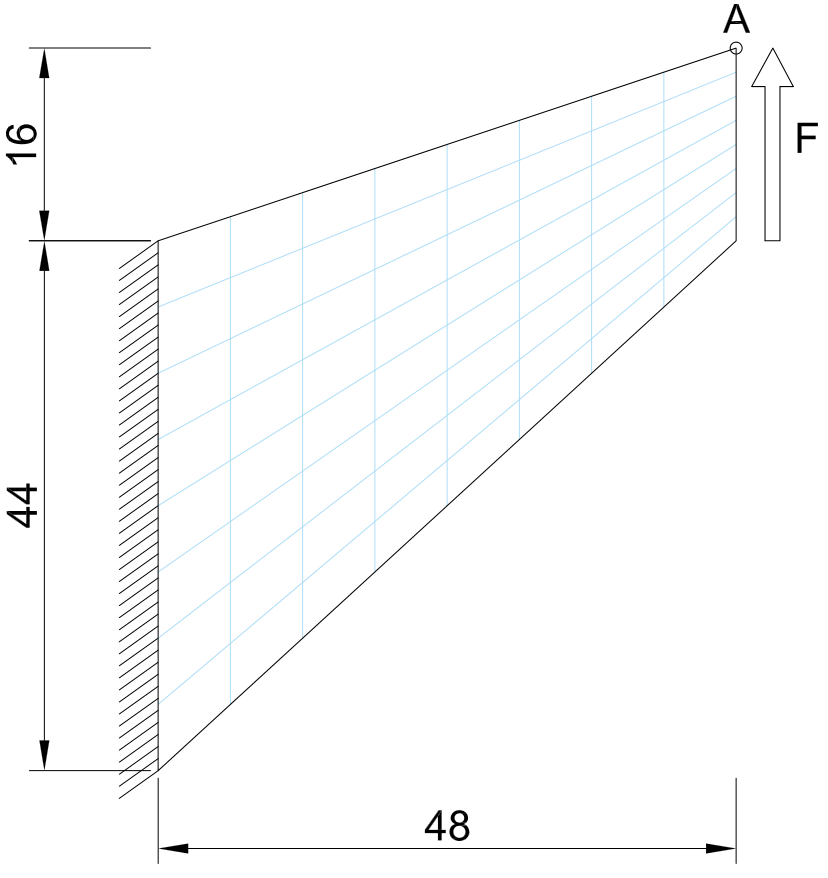
\includegraphics[width=10cm]{membrana8x8.png}
\centering
\end{figure}

\end{document}